\documentclass[a4paper,11pt]{article}
%\addtolength{\parindent}{-5mm%}
%\addtolength{\columnsep}{-5mm}
%\addtolength{\textwidth}{0.5in}
%\addtolength{\hoffset}{-0.5in}
%\addtolength{\textheight}{1in}
%\addtolength{\voffset}{-1in}
\usepackage{cite}
\usepackage{color} 
\usepackage{amsmath}
\usepackage{amsfonts}
\usepackage{amssymb}
\usepackage{amsthm}
\usepackage{graphicx}
\usepackage{hyperref}
\usepackage{amsmath}
\usepackage{amsfonts}
\usepackage{amssymb}
%\hypersetup{
 %  colorlinks, linkcolor={dark-red},
   %citecolor={dark-blue}, urlcolor={medium-blue}
%  }
%\usepackage{hypersetup}
\usepackage[top=0.5in, bottom=0.5in, left=0.25in, right=0.25in]{geometry} 
\begin{document}

\title{ A CS296-28 GROUP REPORT }
\author{
	Avinash\\
	110050064\\
	\href{mailto:bubbu@cse.iitb.ac.in}{bubbu@cse.iitb.ac.in}\\
	\and 
	Nilesh\\
	110050007\\
	\href{mailto:nileshkulkarni@cse.iitb.ac.in}{nileshkulkarni@cse.iitb.ac.in}\\
	\and
	Rajlaxmi\\
	10050087\\
	\href{mailto:rajlaxmisahu@cse.iitb.ac.in}{rajlaxmisahu@cse.iitb.ac.in}\\
	}
\date{\today}
\maketitle
\pagenumbering{roman}
\tableofcontents	
\newpage
\pagenumbering{arabic}
\section{Interesting things about our design}
Our design acts a bit like an "Alarm" with only one snooze step. When the ball which is placed below the pendulum, comes and hits the alarm trigger which enables the alarm.\\
Again after some time we can see that when all the balls fall into the box which is on one-side of the pendulum, the rod rises up and hits the other alarm trigger wh   
\section{Difference between the original and finished design}

\section{Analysis of the code}
\subsection{Plot01 : Step-time Vs Iterative Values}
 	\begin{figure}[ht]
	\begin{minipage}[ht]{0.5\linewidth}
	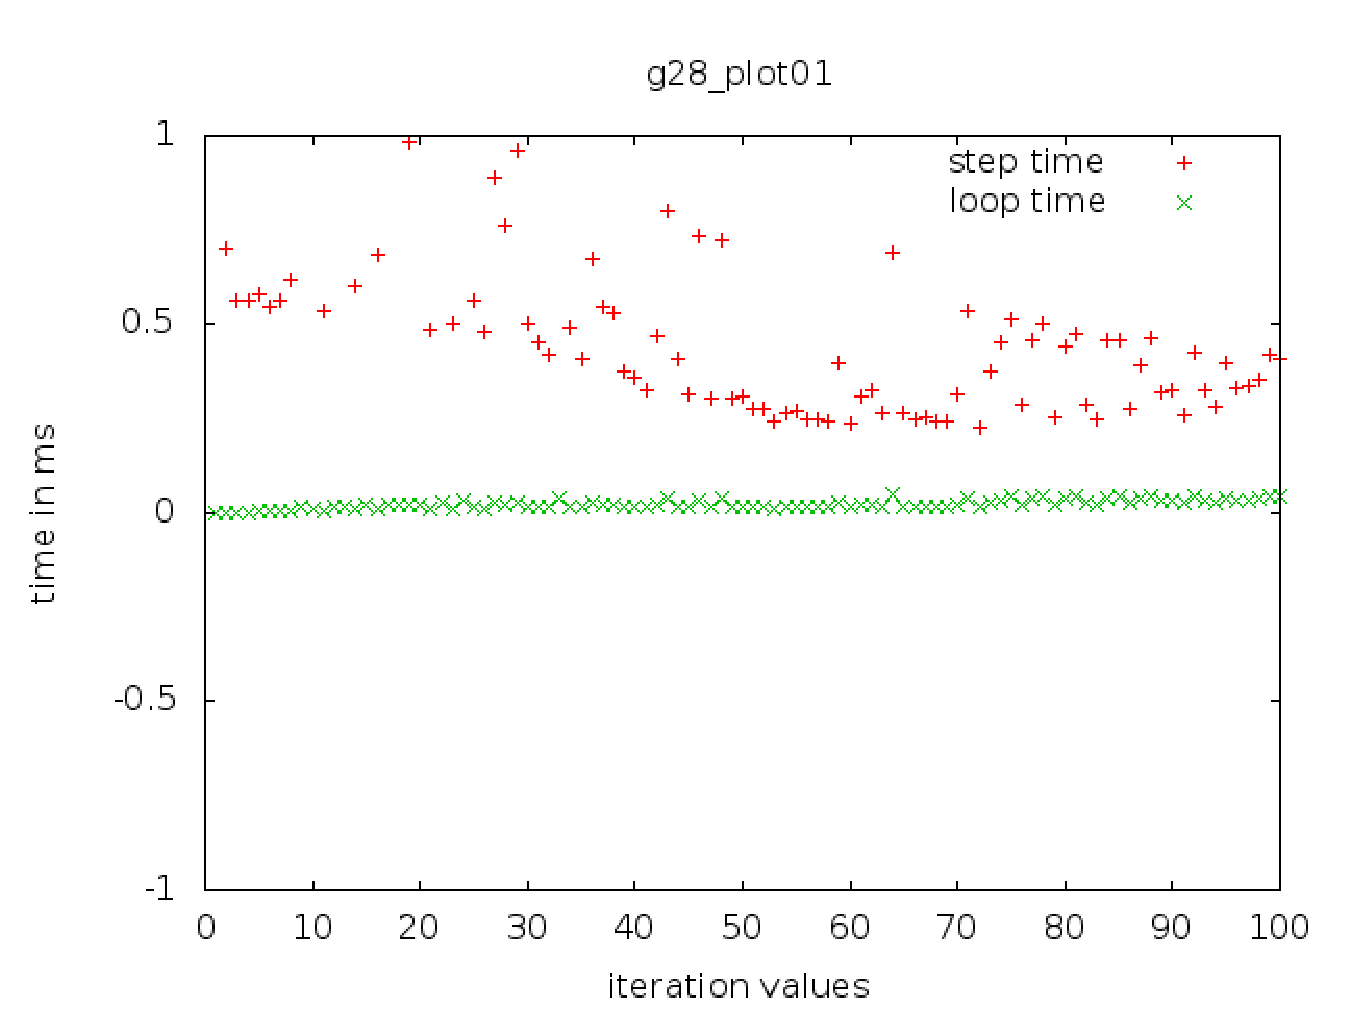
\includegraphics[height=50mm]{plots/g28_plot01.eps}
	\caption{System Resource usage is High }	
	\label{fig:ResourceIntensivePlot01}
	\end{minipage}	
	\begin{minipage}[ht]{0.5\linewidth}
	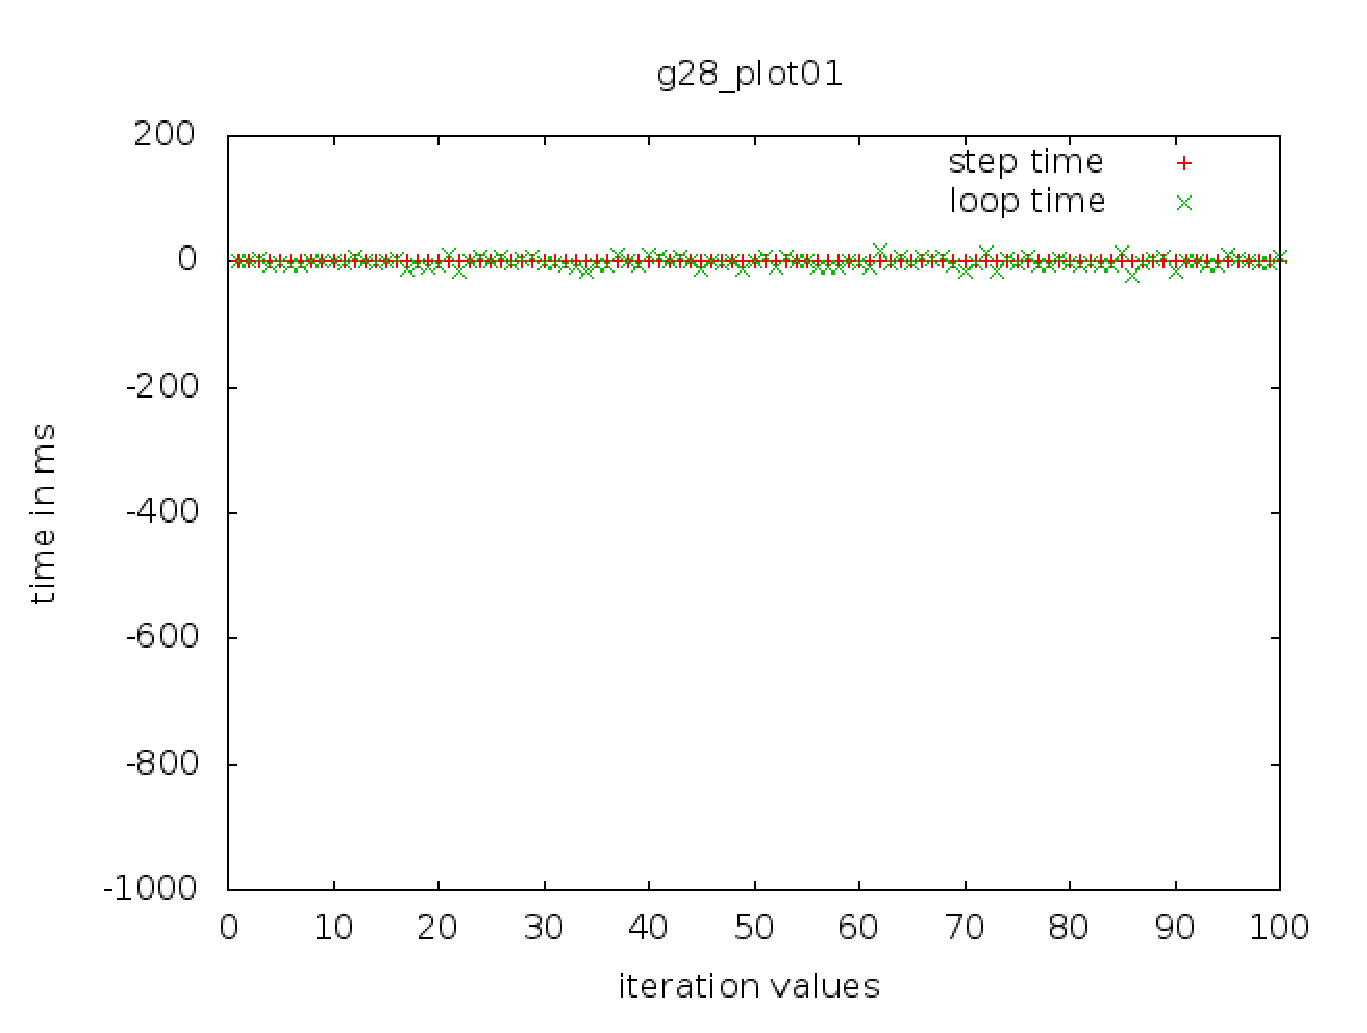
\includegraphics[height=50mm]{plots1/g28_plot01.eps}
	\caption{System Resource usage is Low}
	\label{fig:ResourceIntensivePlot01a}
	\end{minipage}	
	\end{figure}

    Analysis :
\begin{itemize}    
    \item The Step-Time in Figure~\ref{fig:ResourceIntensivePlot01} is totally scattered but the Loop-time is almost
    Linear and the value tends to zero because when the processor is in its full 
    usage, priorities is decided using the scheduling algorithm. So, the running of the base-code is    
    not certain at a given time and so the graph of step-time over Iterative values has no certain pattern.
    \item The Step-Time in Figure~\ref{fig:ResourceIntensivePlot01a} is not scattered and we can see certain decreasing pattern. We can see that the step-time value is large in small number of Iterative-Values and less in the greater range of Iterative-Values, because as the iteration number increase the process becomes more resource intensive and operating system tries to give more resources to such a process(if it can) and hence we observe a decrease in step time. We also feel that as the time for which the process executes increase it gets more CPU resources. 
    \item There is one more interesting observation on the loop time graph which can be divided approximately into two linear graphs,the later one less steeper than the former and the reason for such a behaviour is that the operating system tends to allocate more resources to a program which has been running for a longer time.
    \end{itemize}
  %  \pagebreak
\subsection{Plot02 : Step-Time, Collision-Time ,Velocity-Update ,Position-Update Vs Iterative Values }
	\begin{figure}[ht]
	\begin{minipage}[ht]{0.5\linewidth}
	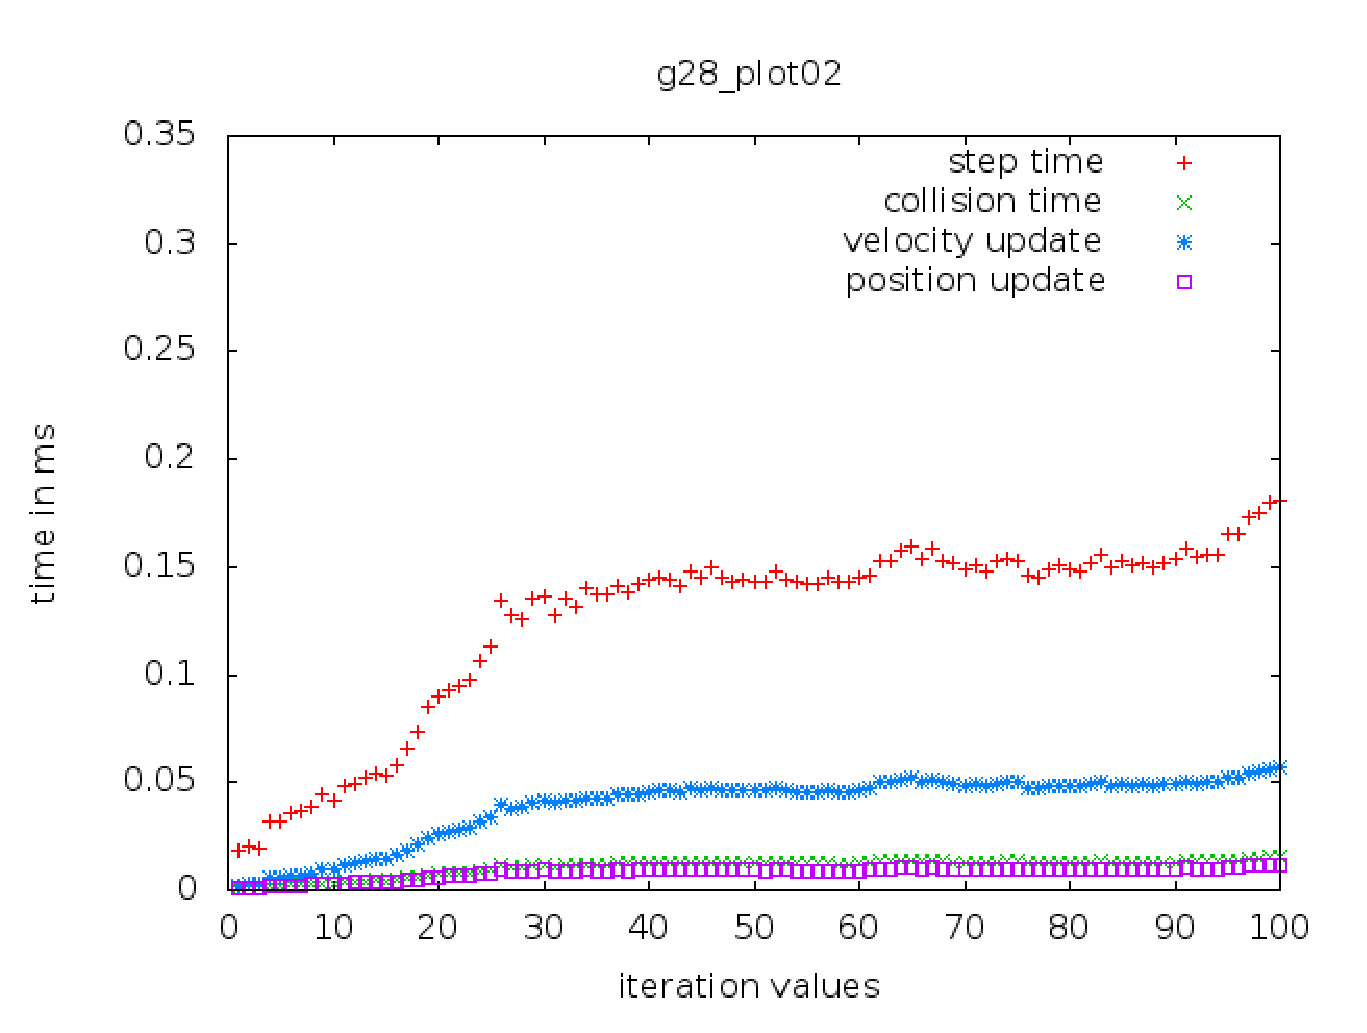
\includegraphics[height=50mm]{plots/g28_plot02.eps}
	\caption{System Resource usage is High}		
	\end{minipage}	
	\begin{minipage}[ht]{0.5\linewidth}
	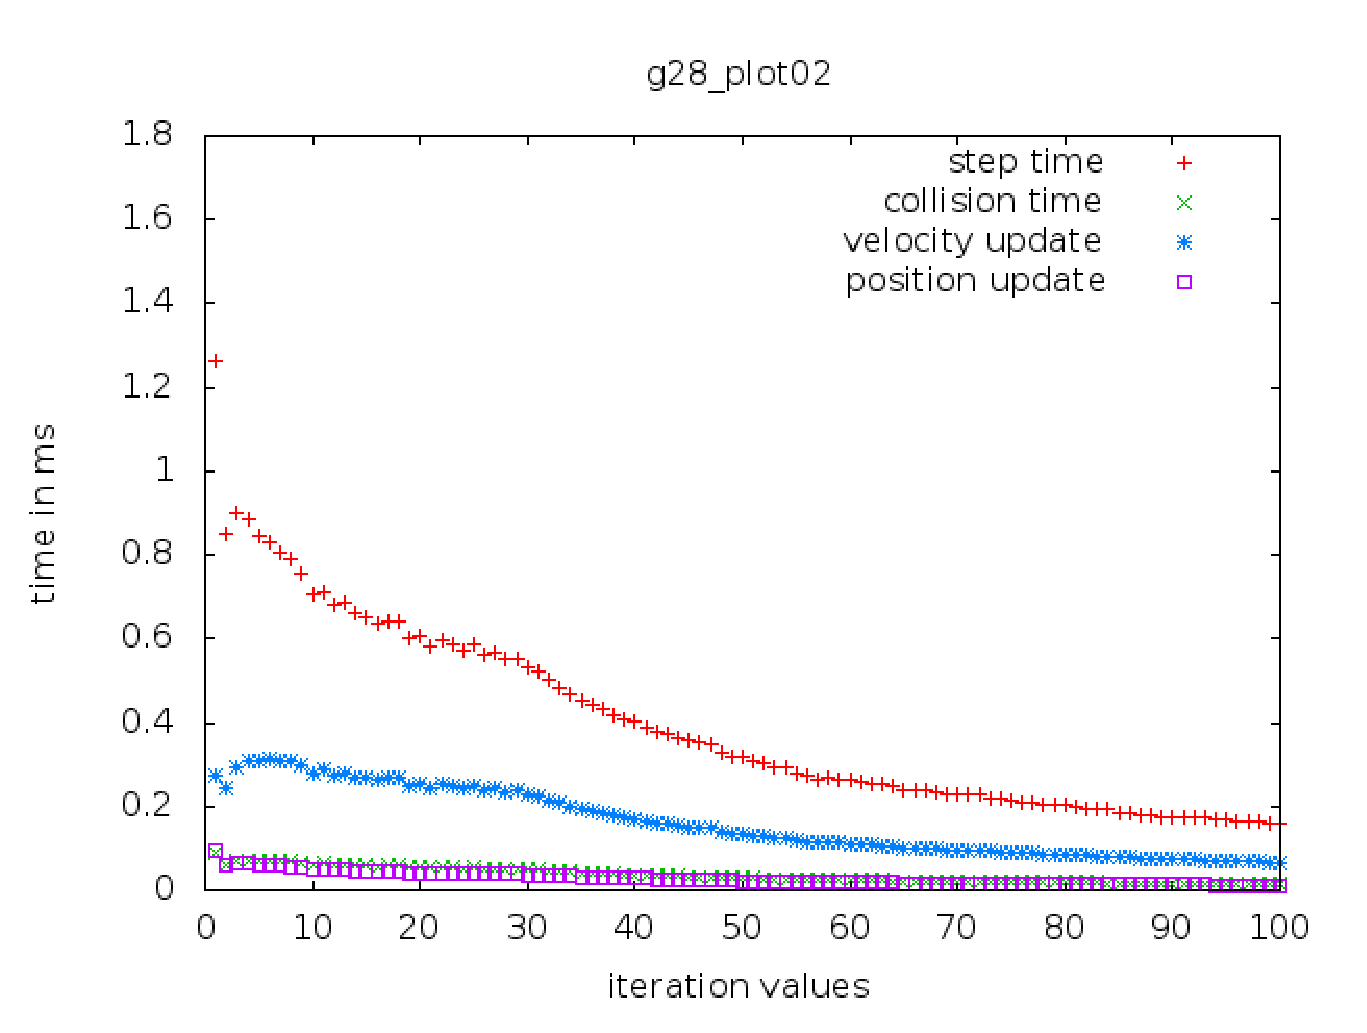
\includegraphics[height=50mm]{plots1/g28_plot02.eps}
	\caption{System Resource usage is Low}		
	\end{minipage}	
	\end{figure}
	Analysis :
\begin{itemize}
\item As the step-time values depend on velocity-update values,the position-update 
 values, collision-time values so as the step-time values are scattered we can easily     
 see that the respective values are also  different at various iterative values.
\end{itemize}
\pagebreak
\subsection{Plot03 : Step-Time, Loop-Time Vs Rerun-Values }

	\begin{figure}[ht]
	\begin{minipage}[ht]{0.5\linewidth}
	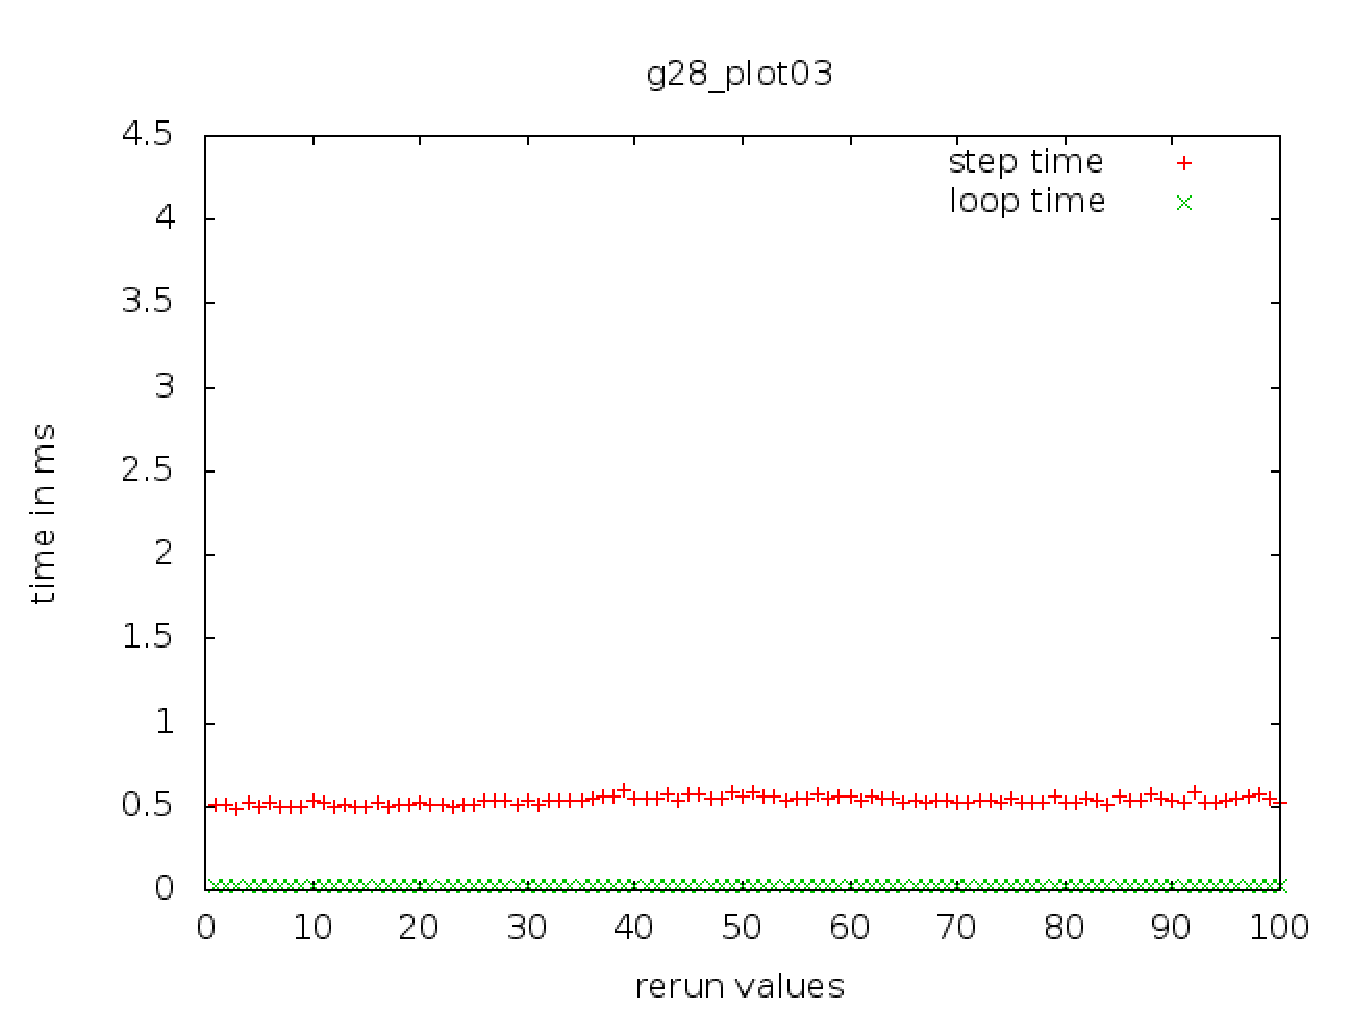
\includegraphics[height=50mm]{plots/g28_plot03.eps}
	\caption{System Resource usage is High}		
	\label{fig:1}
	\end{minipage}	
	\begin{minipage}[ht]{0.5\linewidth}
	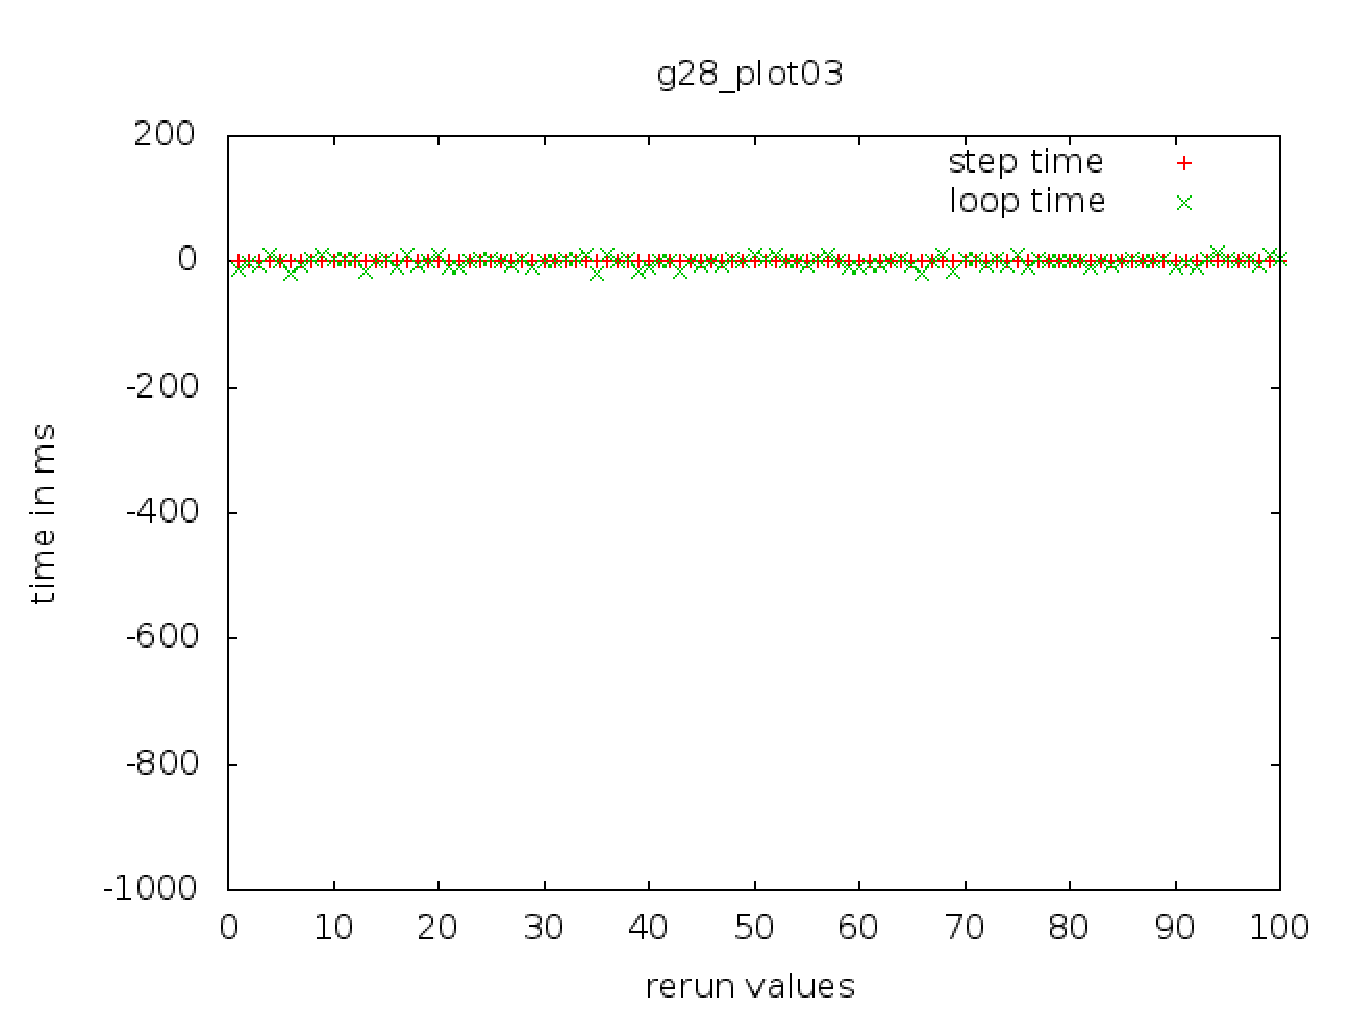
\includegraphics[height=50mm]{plots1/g28_plot03.eps}
	\caption{System Resource usage is Low}		
	\label{fig:2}
	\end{minipage}	
	\end{figure}
	Analysis :
	\begin{itemize}
	\item  We can see that the values of step-time in Figure~\ref{fig:1} are increased, whereas in     
	Figure~\ref{fig:2} are almost equal to zero, the reason is already explained in Figure-1 and Figure-2
	The step time in loaded system 0.5 approximately. This was as expected since the system was loaded.
	\end{itemize}
%	\pagebreak
\subsection{Plot04 : Step-Time, Collision-Time, Velocity-Update, Position-Update Vs Rerun-Values}
\begin{figure}[ht]
	\begin{minipage}[ht]{0.5\linewidth}
	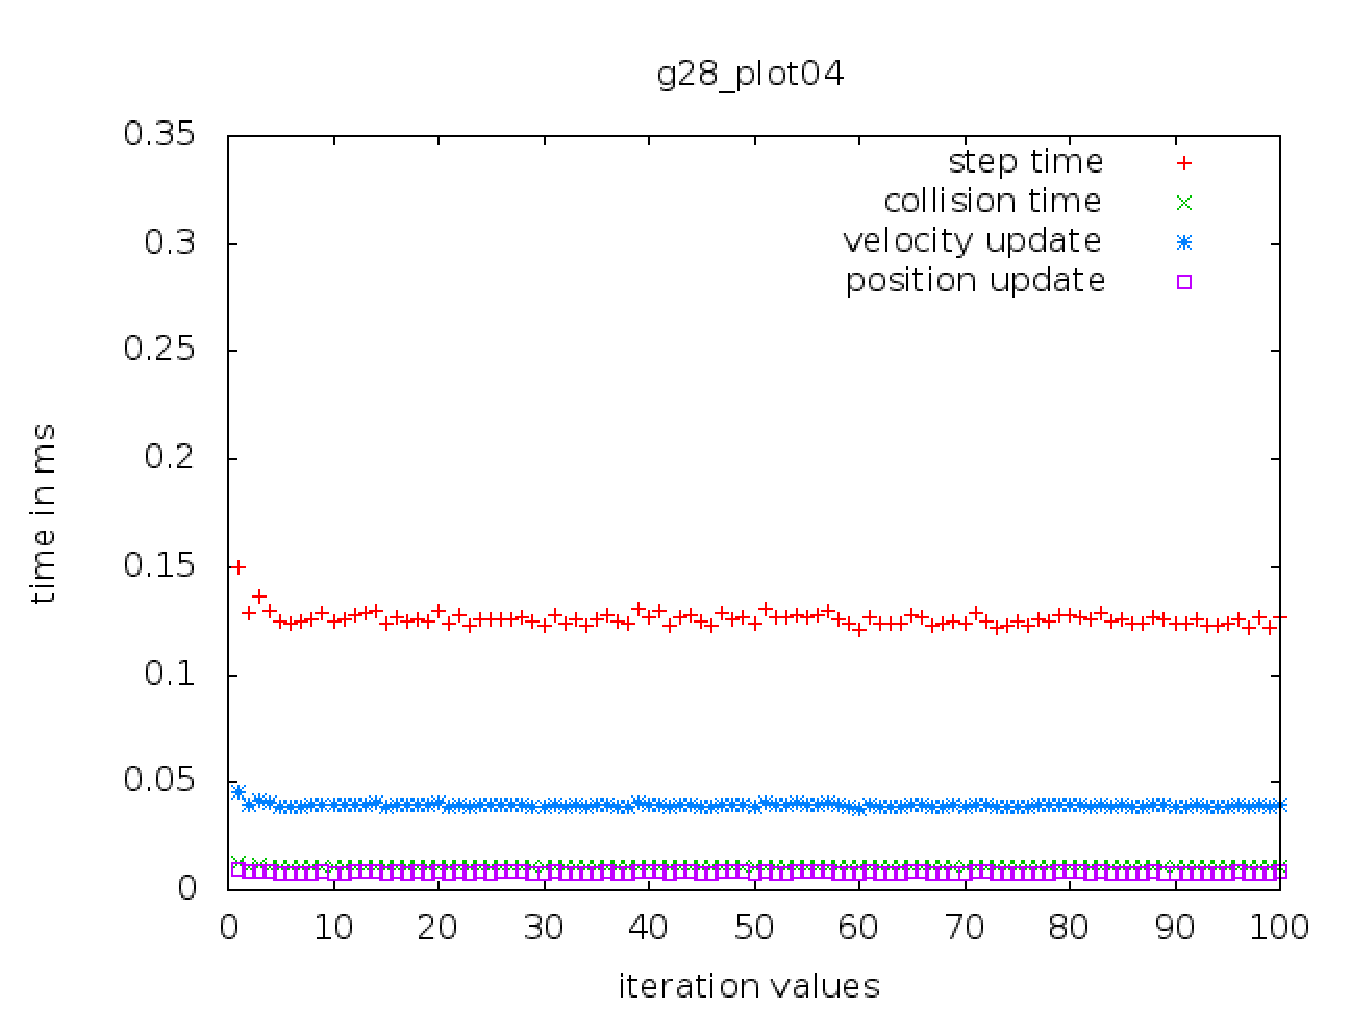
\includegraphics[height=50mm]{plots/g28_plot04.eps}
	\caption{System resources usage is High}		
	\end{minipage}	
	\begin{minipage}[ht]{0.5\linewidth}
	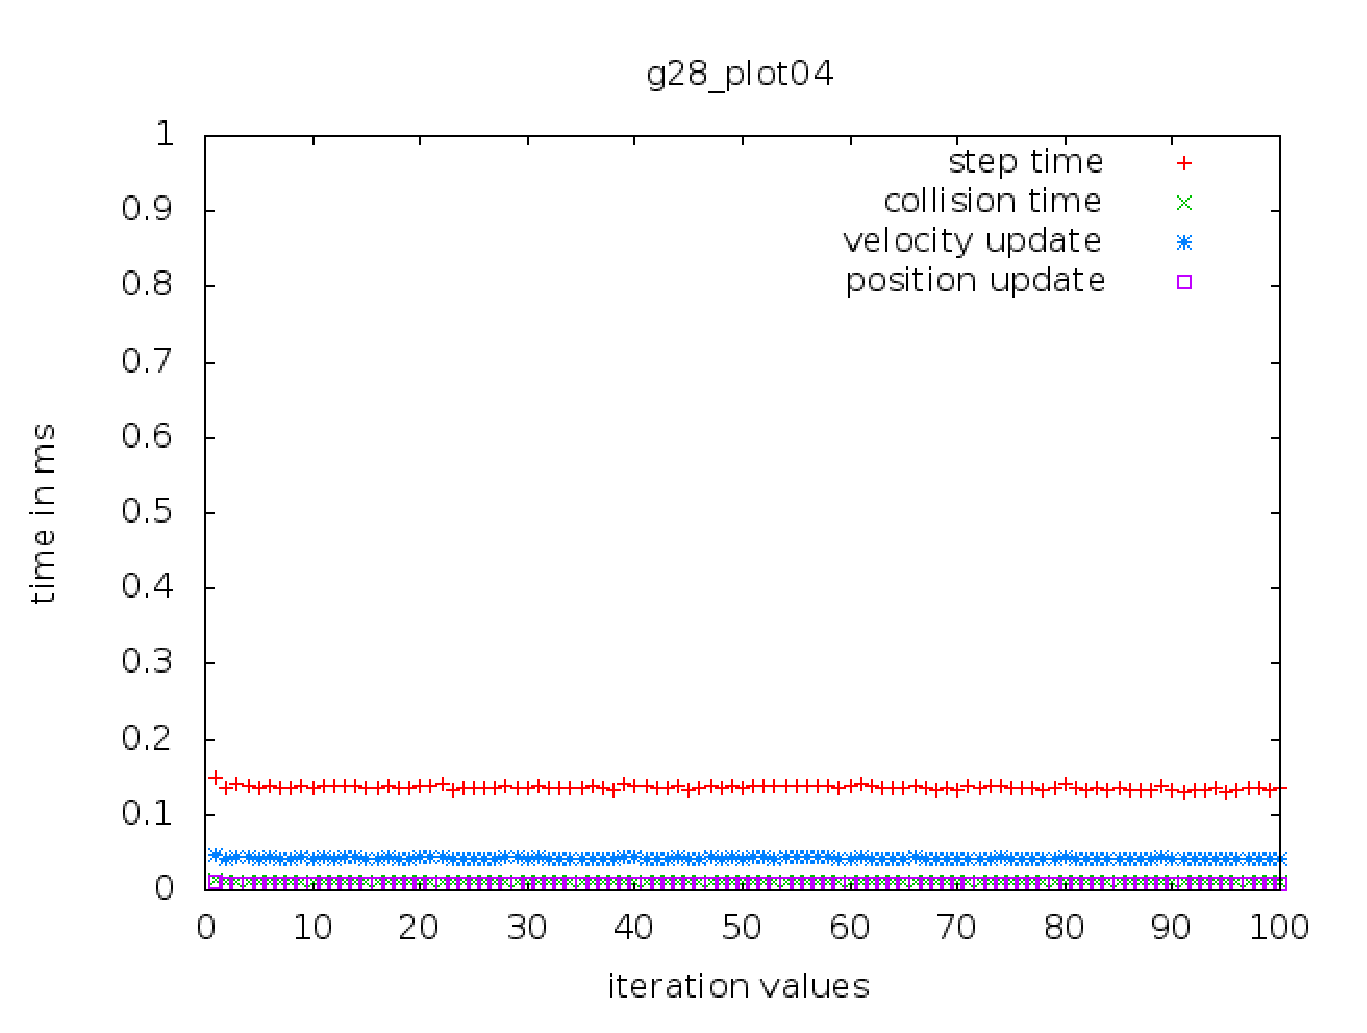
\includegraphics[height=50mm]{plots1/g28_plot04.eps}
	\caption{System Resource usage is Low}		
	\end{minipage}	
	\end{figure}
		Analysis :
	\begin{itemize}
	\item From Plot02 we can see that the step-time values depend on velocity-update 	
	values, the position-update values, collision-time values so an increase in the 
	values of step-time leads to the increase in the values of all the its dependents.
	\end{itemize}
\subsection{Plot05 : Time averaged over all iterative-values Vs Rerun-Values}
	\begin{figure}[ht]
	\begin{minipage}[ht]{0.5\linewidth}
	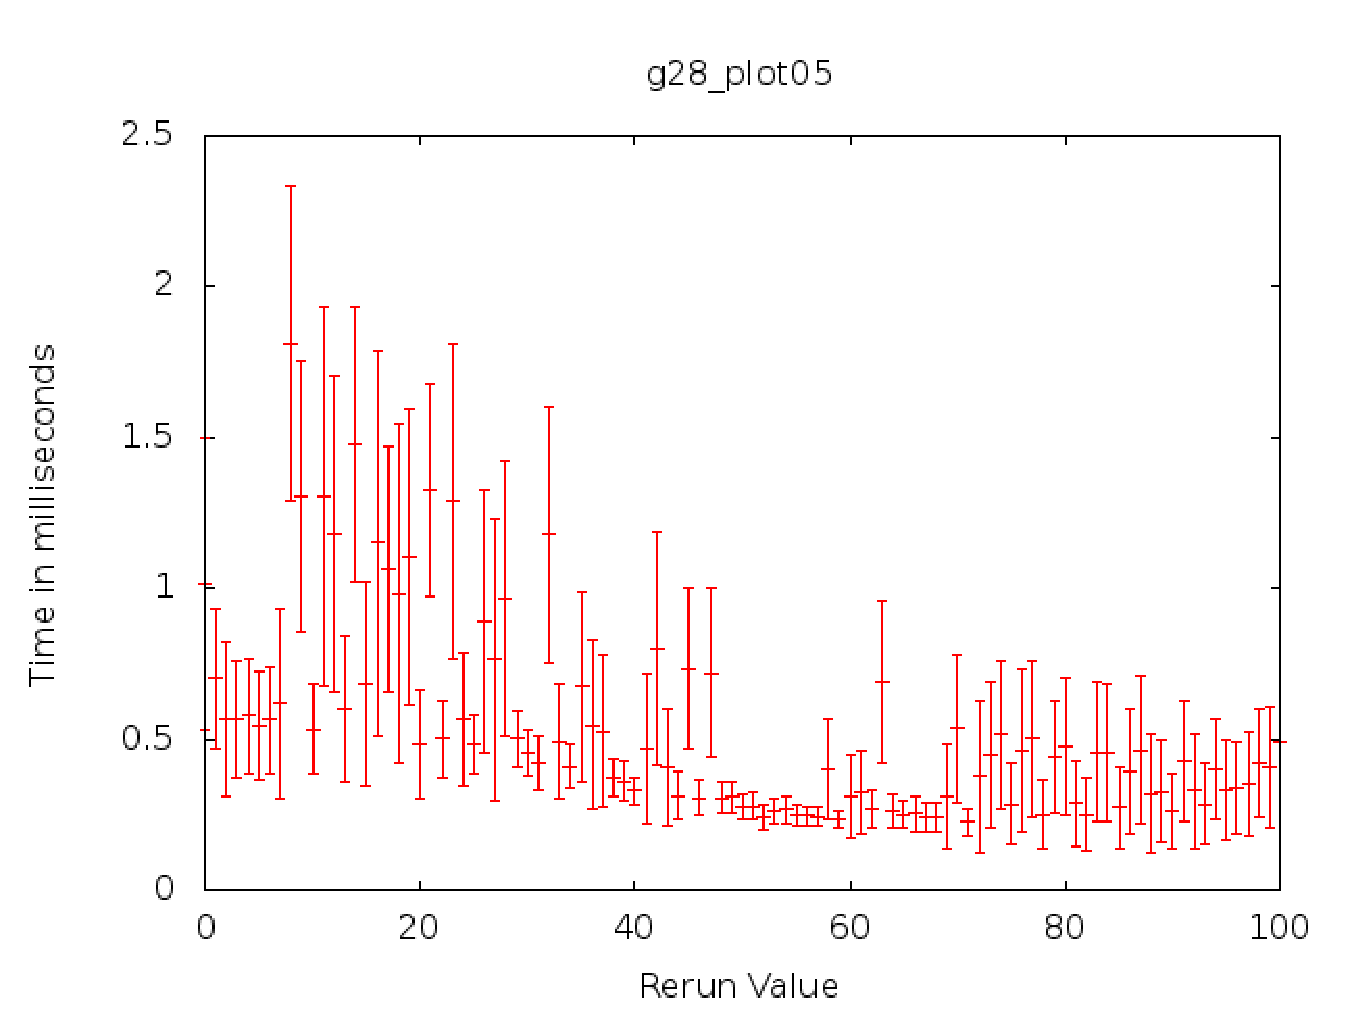
\includegraphics[height=50mm]{plots/g28_plot05.eps}
	\caption{System Resource usage is High}	
	\end{minipage}	
	\begin{minipage}[ht]{0.5\linewidth}
	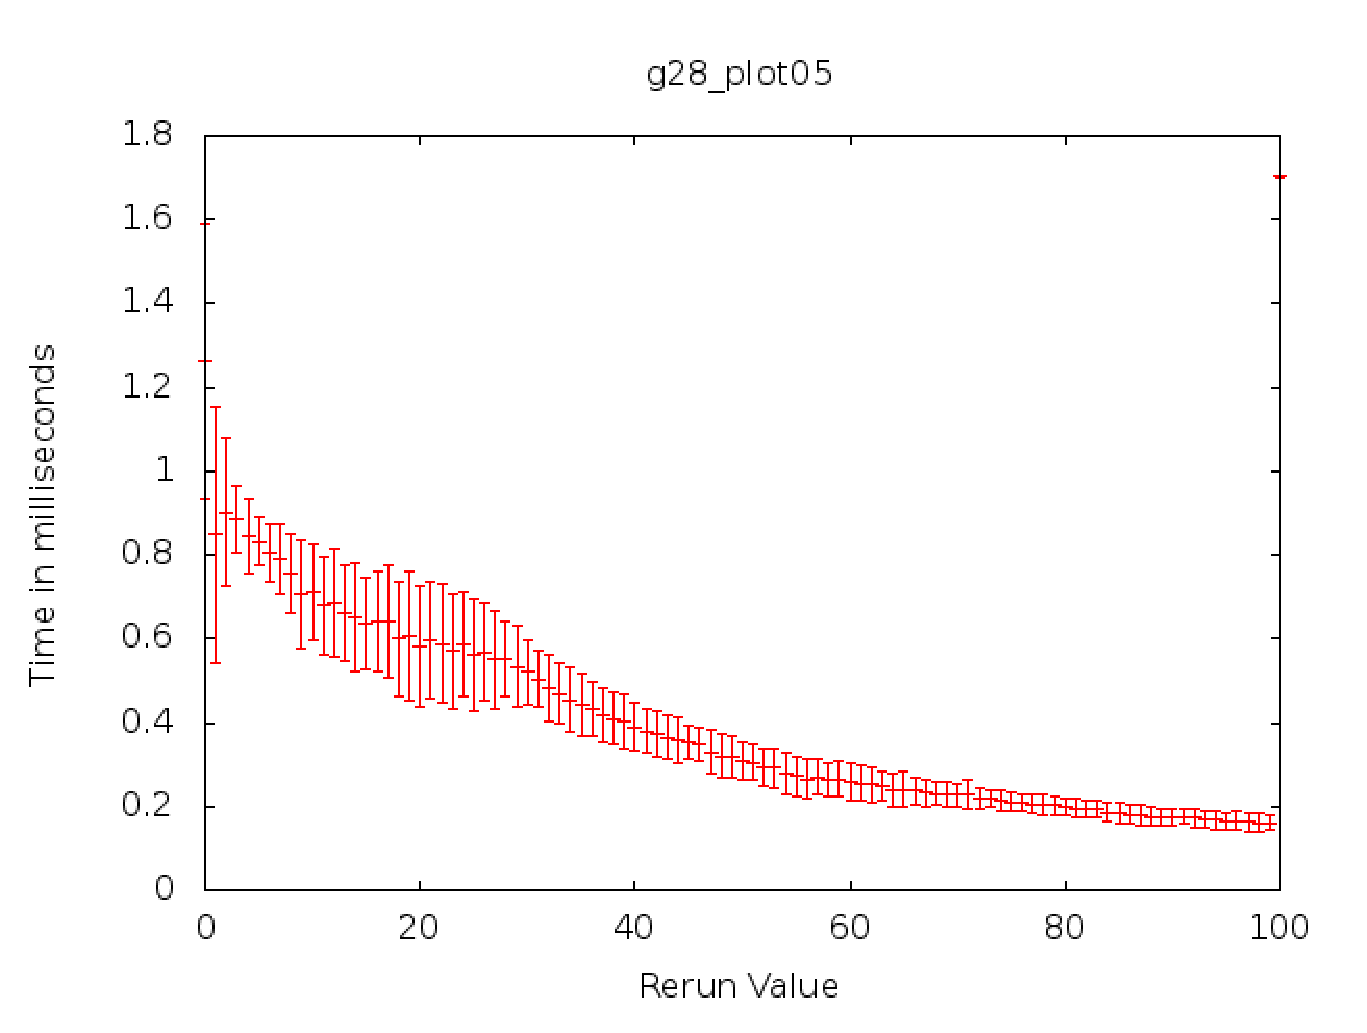
\includegraphics[height=50mm]{plots1/g28_plot05.eps}
	\caption{System Resource usage is Low}		
	\end{minipage}	
	\end{figure}
	Analysis :
	\begin{equation}
	\sigma^2 = \frac{\sqrt{\sum_{i=1}^{N} (x_i -x)^2}}{N}
	\end{equation}
	\begin{itemize}
	\item We can see that as the number of iterative values increases the variance 
	decreases
	\item The values of step-time leads to the increase or decrease in the values of 
	all the its dependents. The variance is inversely proportional to $N$
	\end{itemize}
\subsection{Plot06 : Frequency Vs Step-Time}
\begin{figure}[ht]
	\begin{minipage}[ht]{0.5\linewidth}
	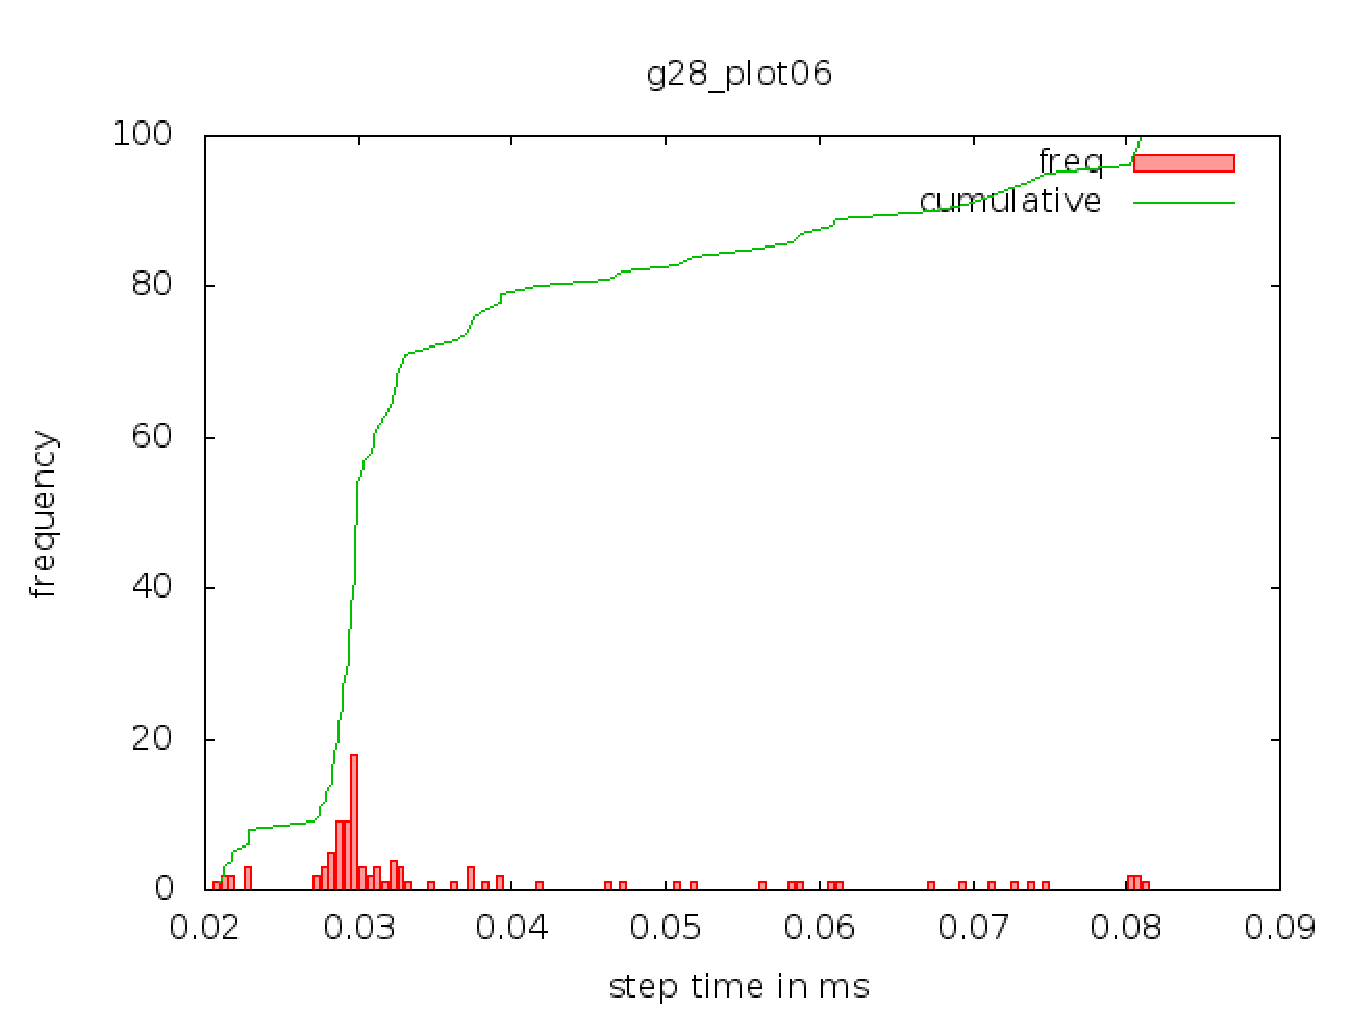
\includegraphics[height=50mm]{plots/g28_plot06.eps}
	\caption{System Resource usage is High}	
	\end{minipage}	
	\begin{minipage}[ht]{0.5\linewidth}
	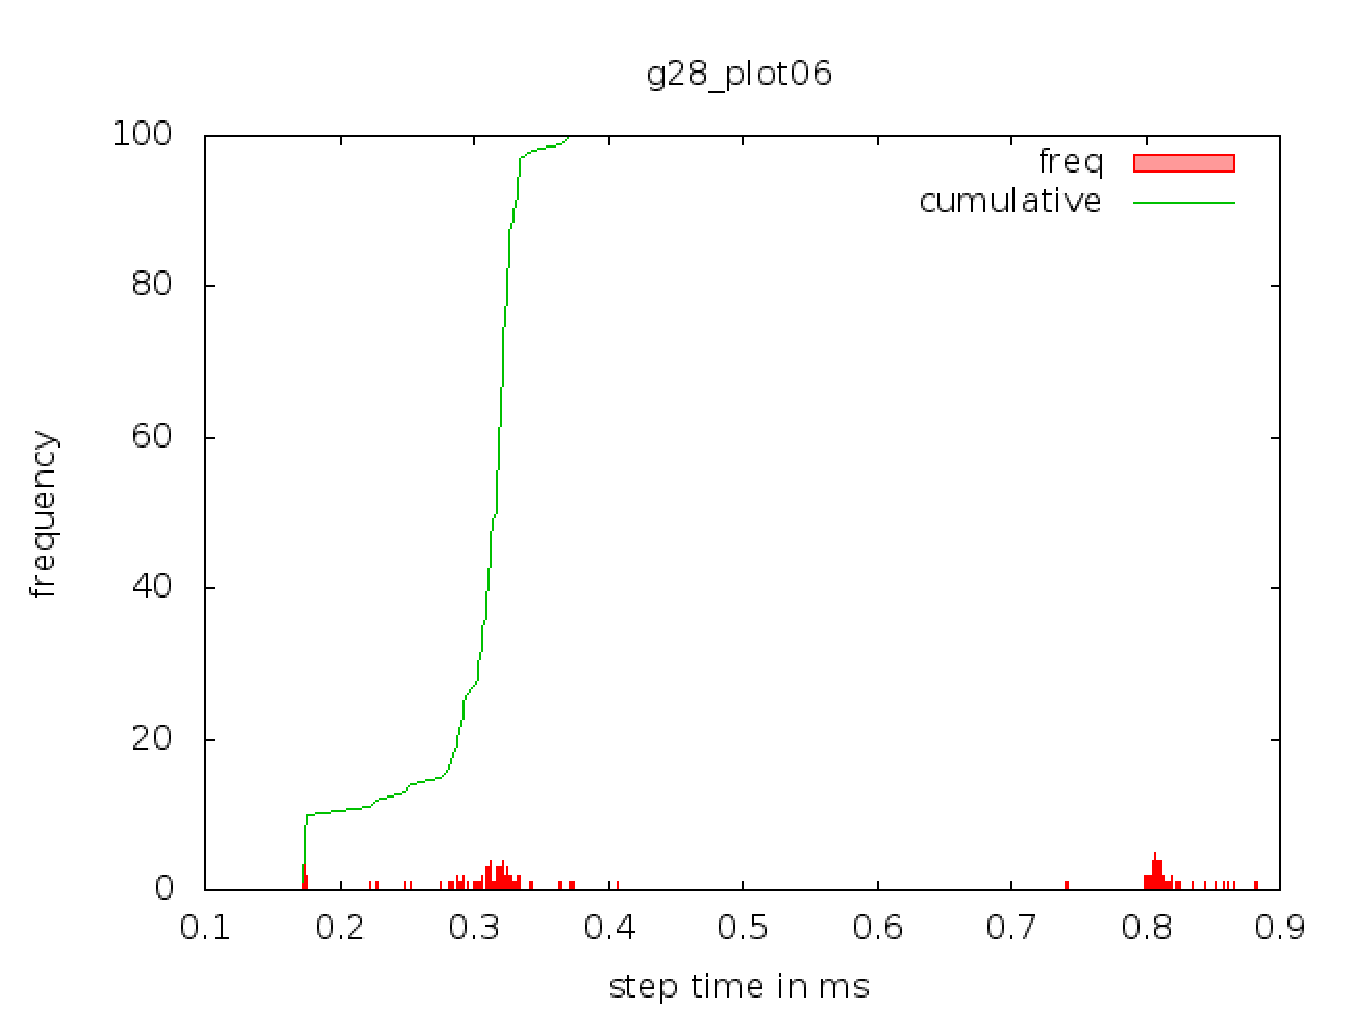
\includegraphics[height=50mm]{plots1/g28_plot06.eps}
	\caption{System Resource usage is Low}		
	\end{minipage}	
	\end{figure}
		Analysis :
\begin{itemize}
\item we can see that there is an increase in the step-time with the increased usage of the System Resource. 
\end{itemize}
\section{Optimization}

O3 and O2 functions optimize significantly which is visible by the time taken i.e 100000 iteration in debug version required 19.77s while release version with optimization turned on required 14.67s.
The functions can be very effectively optimized by inlining i.e. overhead associated with calling and returning from a function can be eliminated by expanding the body of the function inline. This saves a lot of time.\\
\begin{figure}[ht]
	\begin{minipage}[ht]{0.5\linewidth}
	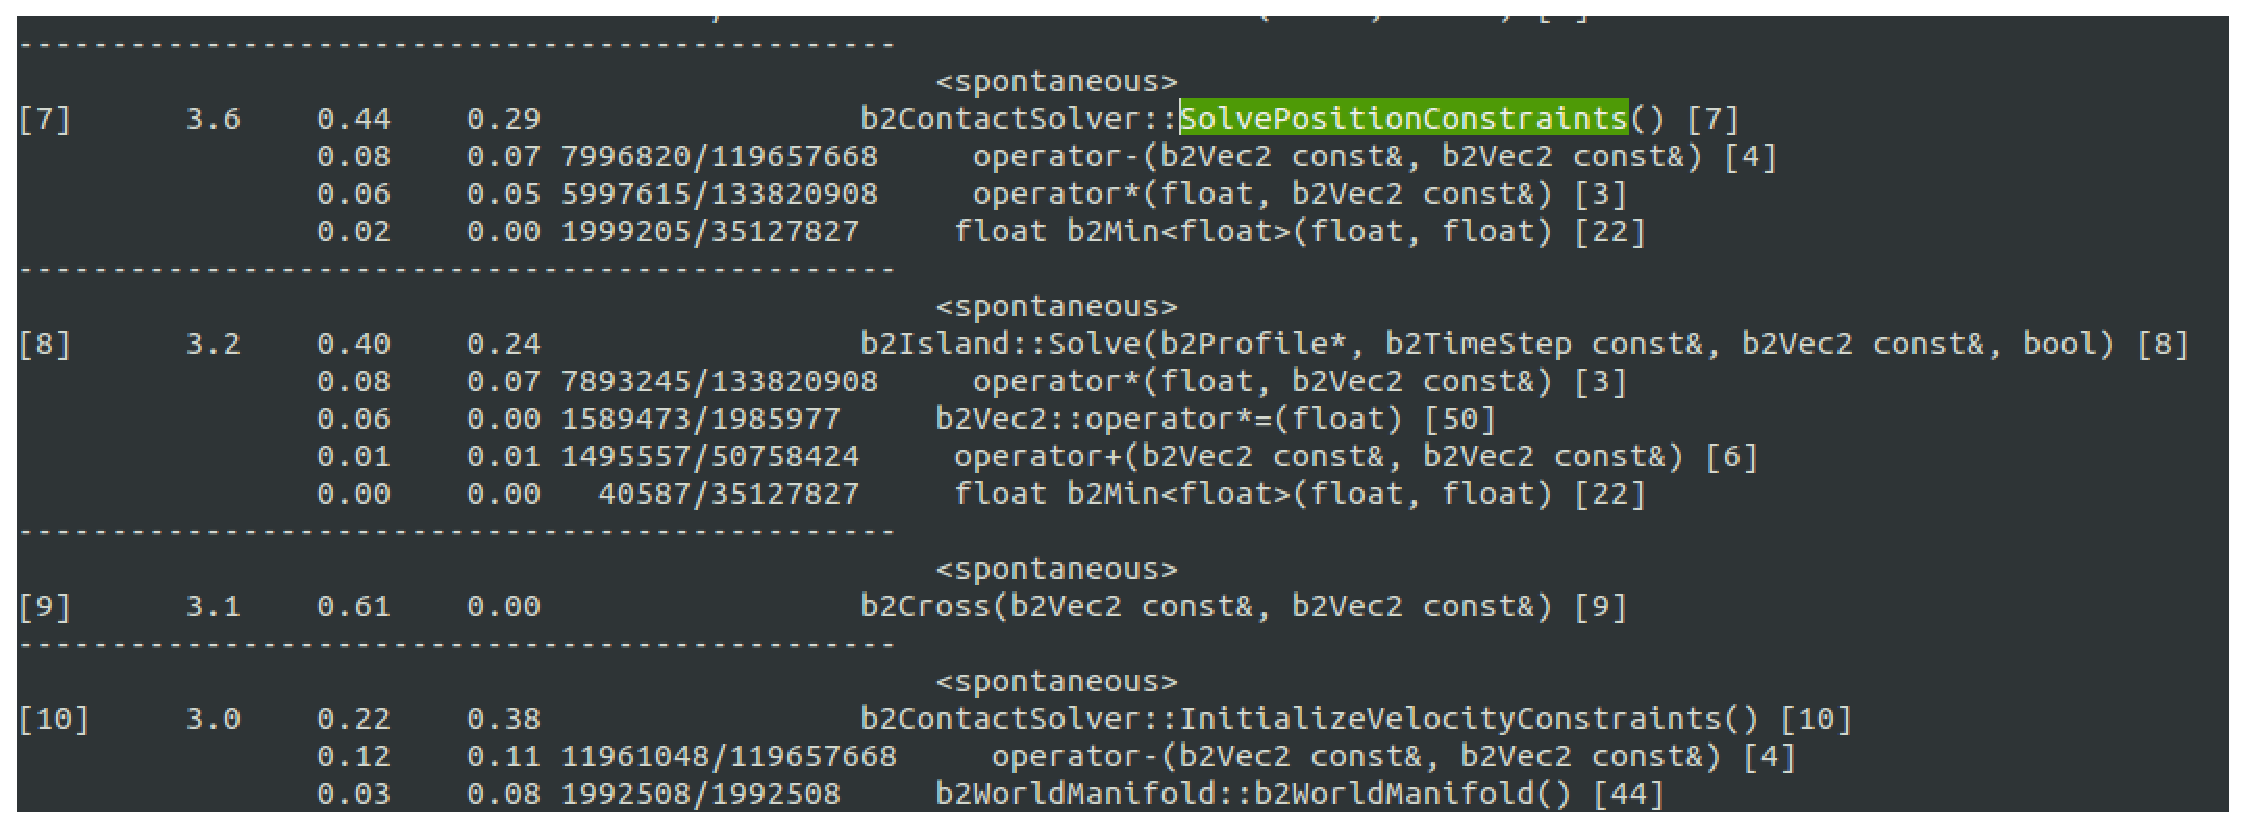
\includegraphics[width=90mm]{1.eps}
	\caption{CallGraph Debug Mode}	
	\end{minipage}	
	\begin{minipage}[ht]{0.5\linewidth}
	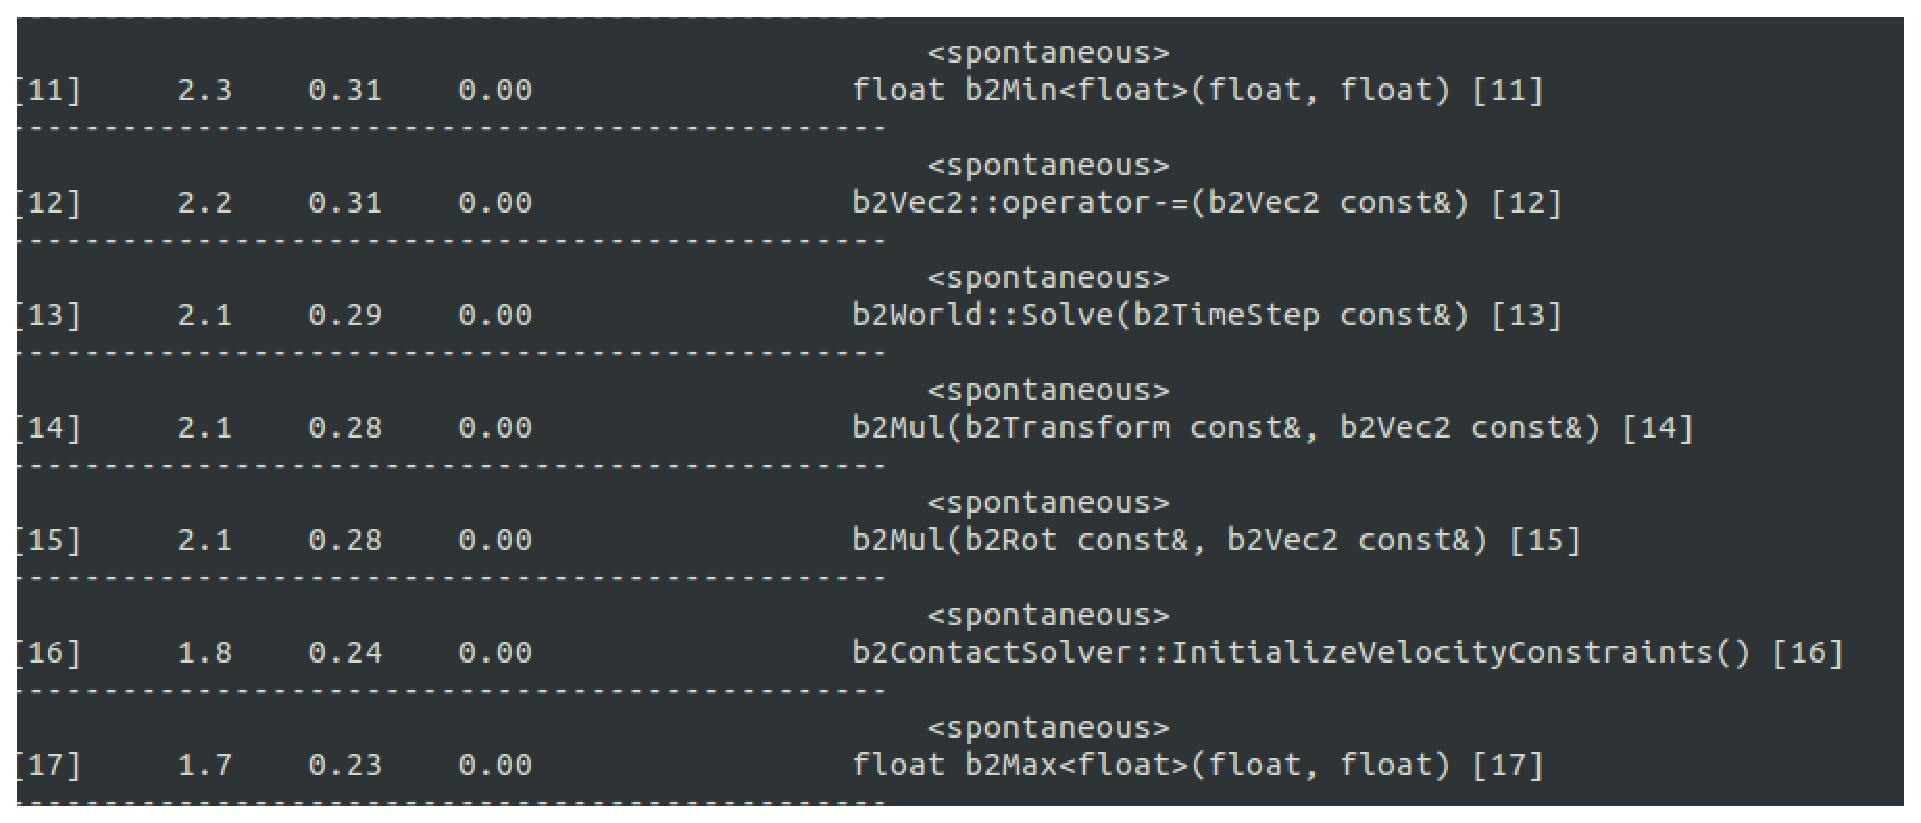
\includegraphics[width=90mm]{2.eps}
	\caption{CallGraph Release Mode}		
	\end{minipage}	
	\end{figure}

In the release-version in-lining of functions is done extensively. This is visible from the profiles generated. In debug version in-lining is not done to analyse the code and make it more readable. This is because one needs to keep a track of all the calls that are generated in order have the debug data.\\


Observe a crucial fact that if the overhead of a calling the function which includes creating a environment, putting the function into the stack etc.. is much greater than the work the functions such functions are called inline while exectuing the code to make it work faster. Such a concept has been applied at many places during release optimization of the code. 
Hence we also observe that the number of functional calls have been significantly reduced due to such a methodology.\\
\begin{figure}[ht]
	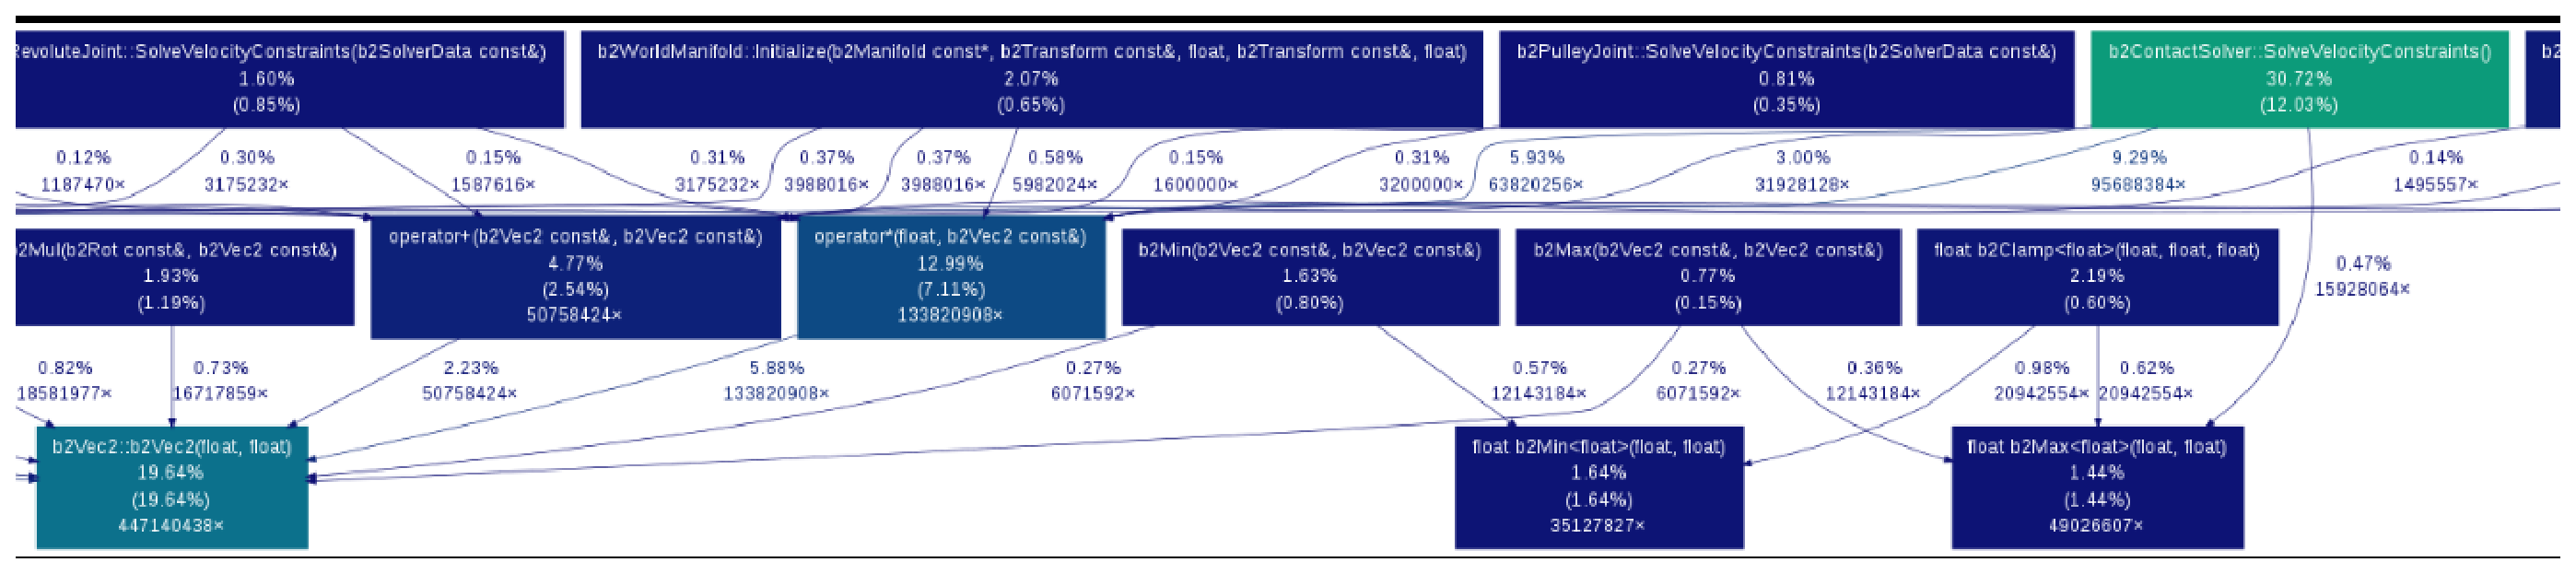
\includegraphics[width=180mm]{3.eps}
	\caption{DebugMode}			
\end{figure}
\begin{figure}[ht]
	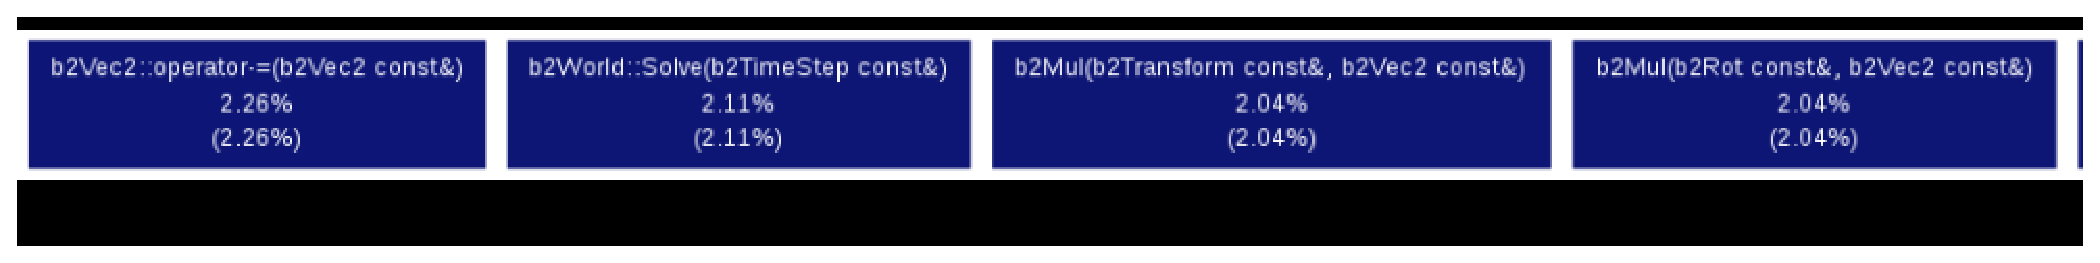
\includegraphics[width=180mm]{4.eps}
	\caption{Release Mode}			
\end{figure}
As visible from a call graph and images in release version, mostly the functions single functions calls.
For example  the b2Vec constructor has been called by various functions which has been  all been turned inline.
Caller-graphs in release version have less number of branches which again shows most of the computation is done in function itself. On the contrary this is not the case in Debug version of the Box2d library and it also turns out the the maximum time is taken up by the constructor( around 15 percent) being such a trivial function with no computation involved.\\
When iteration number are less most of the time goes in initializing and when iteration number are increased then time is mostly spent in distance calculation and then solving velocity constraints surpasses all and requires most time.\\

As visible from profiles basic arithmetic operations * , - and + requires a considerable amount of time. Arithmetic operation are also optimized in optimization for example multiply expressions can be implemented with bit operations. So functions using them also require considerable lesser time as compared to debug version.
\\
Moreover functions are not profiled/tracked when optimizations(especially in the release version of the code) are turned on which also contributes to a very high efficiency
\\
\section{Project Code Which Can Be Optimized}
\begin{itemize}
\item In b2ContactSolver.cpp line number 317, 402, 403 multiple calls to $vc->points$ in each loop can be saved instead of calling in each loop.

\item Instead of calling mathematical functions like b2Dot and b2cross we can use those function description inline.
For example: 
\begin{verbatim}
b2Vec2::b2vec(float x ,float y)
{
	x=x; y=y;
}
\end{verbatim}
We can make  this function inline and reduce the overhead

\item For gdb to support inlined functions, the compiler must record information about in-lining in the debug information. So in debug version inline (definition is excluded.
\end{itemize}

\end{document}
